% Here is a suggested template for PhD research proposal for the
% first annual report.
% Written originally 2010-06-22 by T. W. Yee.
% Last modified      2010-07-22 by T. W. Yee.


\documentclass[12pt,a4paper]{article}

\usepackage{natbib}    % For BibTeX
\usepackage{graphicx}  % To import .pdf files
\usepackage{caption}
\usepackage{subcaption}
\usepackage{booktabs}
\usepackage{comment}
% \usepackage{times}
\usepackage{setspace}
\onehalfspacing
% \doublespacing

\oddsidemargin  -10mm
\evensidemargin -10mm
\headheight 0mm
\headsep -3mm
\textheight 250mm
\textwidth 180mm
\topmargin -4mm
\topskip -10mm

%\textwidth=450pt
%\hoffset=-2cm

\usepackage{amsmath}
\usepackage{amsfonts}
\newcommand{\bu}{\boldsymbol{u}}
\newcommand{\bx}{\boldsymbol{x}}
\newcommand{\by}{\boldsymbol{y}}
\newcommand{\bz}{\boldsymbol{z}}
\newcommand{\bY}{\mathbf{Y}}
\newcommand{\bX}{\mathbf{X}}
\newcommand{\bZ}{\mathbf{Z}}
\newcommand{\btheta}{\boldsymbol{\theta}}
\newcommand{\mat}[1]{\mathbf{#1}}

\usepackage[acronym]{glossaries}
\newacronym[shortplural={ATIS}]{atis}{ATIS}{advanced traveller information system}
\newacronym{avl}{AVL}{automatic vehicle location}
\newacronym{apc}{APC}{automatic passenger counter}
\newacronym{rti}{RTI}{real-time information}
\newacronym{gps}{GPS}{Global Positioning System}
\newacronym{api}{API}{application programming interface}
\newacronym{gtfs}{GTFS}{general transit feed specification}
\newacronym{knn}{KNN}{$k$-nearest neighbour}
\newacronym{ann}{ANN}{artificial neural networks}
\newacronym{svm}{SVM}{support vector machines}
\newacronym{kf}{KF}{Kalman filter}
\newacronym{pf}{PF}{particle filter}
\newacronym{mcmc}{MCMC}{Markov chain Monte Carlo}
\newacronym[longplural={expected times of arrival}]{eta}{ETA}{expected time of arrival}
\newacronym{at}{AT}{Auckland Transport}
\newacronym{pt}{PT}{public transport}
\newacronym{ui}{UI}{user interface}
\newacronym{sir}{SIR}{sampling importance resampling}

\newcommand{\kf}{Kalman filter}
\newcommand{\pf}{particle filter}



\usepackage[hidelinks]{hyperref}
\usepackage{cleveref}


\begin{document}

\begin{Large}
\begin{center}
\textbf{Real-time prediction of bus arrival} \\
\textbf{by Tom Elliott} \\
\textbf{for a PhD in Statistics}
\end{center}
\end{Large}


\hfill{Student ID: 1596870}

\hfill{Email: tom.elliott@auckland.ac.nz}

Supervisor: Professor~T.~Lumley

% Co-supervisor: Dr~B.~Brewer

% Advisory Committee: Drs~B.~Efron, D.~R.~Cox, K.~Pearson.\footnote{
% Specify the affiliation if outside the UoA Statistics
% Department.}



\begin{center}
\today
\end{center}


This document represents the student's research proposal after
one year of provisional PhD registration.
Confirmed PhD registration is now sought.




% ----------------------------------------------------------------------
\section{Introduction}
\label{sec:intro}

Something about public transport being important to running of a city, transport, etc.
In order to attract greater ridership, many agencies have deployed \glspl{atis}
to make public transport a more appealing option for commutes.
One major component of \gls{atis} is provision of \gls{rti}, 
in particular arrival time information, 
which usually comes in the form of a countdown display at stops
\citep{cn}.
Several studies have shown that in the presence of real-time arrival information, 
passengers perceive shorter waiting times (time passes more quickly), 
and are generally more accepting of having to wait at the bus stop
\citep{tcrp:2003}.


\gls{rti} goes a lot further than just a countdown at a bus stop,
and can be very useful for passengers trying to plan their journey.
For example, they can find out before heading to the bus stop what time it will arrive,
enabling them to time their arrival to reduce waiting time.
Additionally, they may need to arrive before (or after) a specific time,
so consulting \gls{rti} can help them in deciding which bus to catch.
This all becomes especially useful when there are significant delays in the system.


Of course, in order to provide \gls{rti}, 
transit companies first need to deploy certain technologies to make it possible.
The main technology responsible for \gls{rti} is \gls{avl},
which allows tracking of transit vehicles in real-time.
This location information can then be used to determine the state of a vehicle,
for example speed and position along a route,
which is in turn used to predict arrival times at stops further along the route.


Another use for \gls{avl} information is for developers of public transport apps,
such as the \emph{Track My Bus} app \citep{trackmybus},
which is yet another form of \gls{atis}.
One common way of providing data to developers is through an \gls{api},
such as \gls{gtfs}, which is a globally use format for providing transit data,
including real-time vehicle locations, to developers, 
and is used by Auckland Transport.


Somehow transition from \gls{avl} to modeling.
Over the years, many models have been implemented that use a variety of \gls{avl} technologies
targeting a range of different applications.
Early works, such as those of \cite{wall-dailey:1999} and \cite{dailey:2001},
used the \kf{}, which is ideal for real-time applications, including tracking and navigation,
due to its speed and low computational requirements.
Other research has focused on data-driven models,
most notably \gls{ann} and \gls{svm}, 
which were found to provide more accurate predictions for stops further ahead,
compared to the \kf{} which is typically only able to predict a few stops ahead
\citep{cn}.


Recently, the \pf{} has been used in transit applications \citep{cn},
now more viable for real-time applications thanks to the advancement of 
computer processing power.
The key benefits of the \pf{} are that it allows a more explicit specification of the model
and makes far fewer assumptions than the \kf{},
giving it the potential to overcome many of the problems affecting other transit models.


Within the Auckland Transport system, there are several key issues we hope to overcome.
The first of these is prediction inaccuracy, 
which typically presents as sudden changes in \glspl{eta}.
Another issue is the underlying model estimating the actual position of transit vehicles,
made most evident at loops, in which, given a coordinate, 
a bus could be either heading into or out of the loop,
as shown in \cref{fig:colwill-loop}.
In this case, a passenger may believe they have missed their bus and head home until the next one.
Finally, there is driver error, specifically when entering the wrong route number,
and major delays, which,
from our point of view, present the same,
however they have different implications.


\begin{figure}[!b]
  \centering
  \begin{subfigure}{0.4\textwidth}
    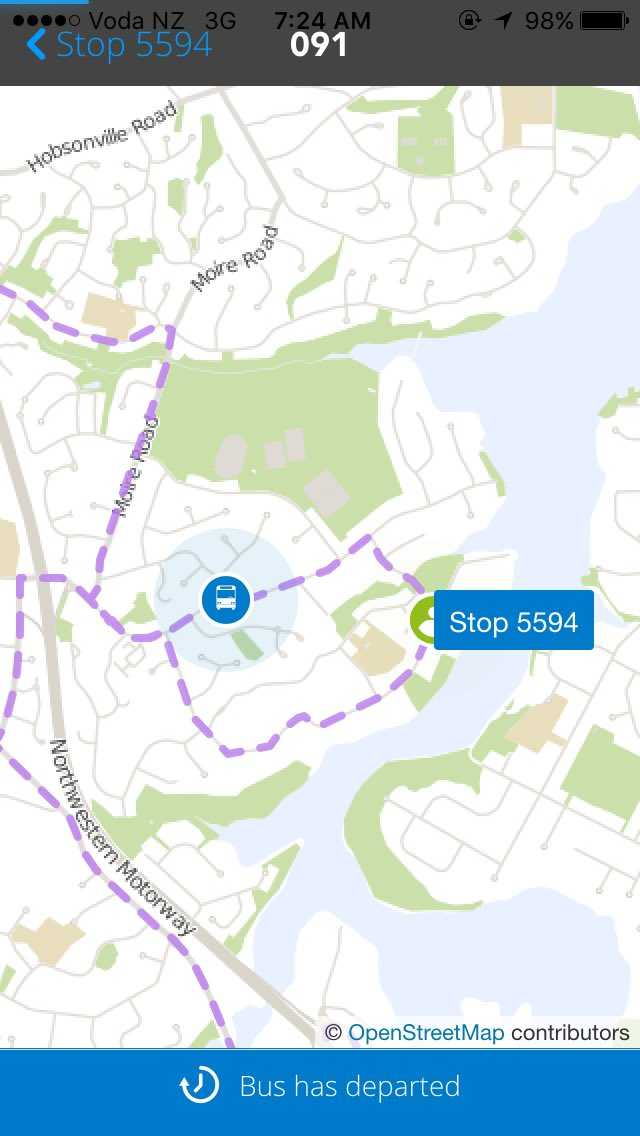
\includegraphics[width=\textwidth,trim={0 0 0 15cm},clip]{bus-loop-durp1.jpg}
    \caption{7:24~am}
    \label{fig:colwill-loop-1}
  \end{subfigure}
  ~
  \begin{subfigure}{0.4\textwidth}
    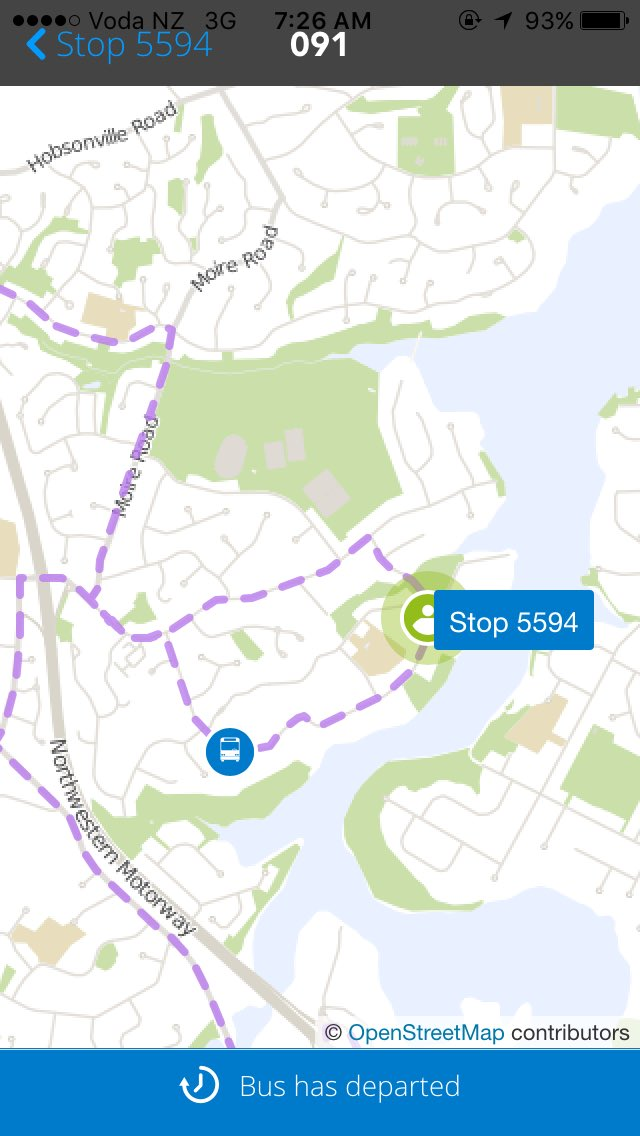
\includegraphics[width=\textwidth,trim={0 0 0 15cm},clip]{bus-loop-durp2.jpg}
    \caption{7:26~am}
    \label{fig:colwill-loop-2}
  \end{subfigure}
  \caption{%
    The scheduled arrival time at stop~5594 is 7:24~am, 
    and the loop runs anti-clockwise.
    The bus position was wrongly estimated in (a), 
    implying to the passenger that they had missed their bus. 
    Note that, even when the bus is positioned correctly on the route in (b), 
    the status is still \emph{departed}, 
    which implies that the underlying model is unable to correct itself in this situation.\newline
    \footnotesize{[Screenshot taken from \emph{Track My Bus} \citep{trackmybus}].}}
  \label{fig:colwill-loop}
\end{figure}


Our primary goal is to implement a \pf{} to the \gls{avl} data provided by Auckland Transport
that can accurately model buses in Auckland, 
and also overcomes the issues mentioned above.
We will then explore ways of incorporating the real-time state of all other buses in Auckland
simultaneously to increase the accuracy and precision of arrival time estimates.
Lastly, we will investigate several applications of our prediction model:
the first will be to provide useful prediction intervals to passengers
(who we cannot assume to have any understanding of the concept of a 
``confidence'' or ``credible'' interval),
and secondly a journey planning application which allows passengers to enter their destination
and be provided with the ``best'' route to take home.

% ====================================================================================================== % INFO

% This document is a template that can be edited by the student.
% Fill in the details as you go along and delete these instructions.
% Do have your research proposal scrutinized by your supervisor before
% submitting it to the department.



% Give a few paragraphs here on the general background
% to your research proposal; put the full details in
% Section~\ref{sec:background}. You might want to cite a few
% previous important results/papers. Describe any theory briefly
% here but put most of the details in Section~\ref{sec:background}.
% Describe any data in general with a few lines here but put the
% full details in Section~\ref{sec:data}.


% Motivate this section well \ldots why is the topic important?
% What use will the thesis have?
% What is unknown that will be known upon completion?


% This section should be understandable by an intelligent person
% who is not familiar with the technical details involved.
% The reader should be convinced that your work
% is worthwhile.





% Some of our PhD students have published in the primary literature
% directly using material from their thesis,
% e.g.,
% \cite{wors:1979},
% \cite{yee:wild:1996},
% \cite{wild:yee:1996},
% \cite{murr:1999},
% \cite{jian:scot:wild:2006},
% \cite{roev:meye:etal:2007},
% \cite{mill:stew:2007},
% or submitted such as
% \cite{lee:hiro:2008}.
% Ideally you should aim at least one of your publications towards
% a mainstream statistics journal, preferably your first one.
% All publications should be in a peer-reviewed international journal.
% It should be in the primary literature.
% Statistical theory and methodology is to be regarded as the highest
% form of quality output.
% Accompanying high quality software that can easily be used
% by others (such as a R package) is also good.
% It is best to submit to journals before the completion of a thesis
% because an acceptance validates the quality of that research.



% A word about writing up your thesis.
% In general, the Department of Statistics recommends \LaTeX{} rather than
% Microsoft Word.
% \LaTeX{} is easily run on the Department's Linux machines.
% A website that converts pdf into Word is \textsf{www.pdftoword.com}.
% The University of Auckland offers a half-day workshop
% on \LaTeX{} to postgraduate students.
% There is Sweave \citep{lmucs-papers:Leisch:2003b} which allows R
% \citep{R:Ihaka+Gentleman:1996} to be embedded into a \LaTeX{}
% document, and so the output does not have to be manually
% cut-and-pasted in. Sweave is useful for presentations too,
% in conjunction with Beamer.


% There is an editor called Emacs which is useful for all types of
% editing, including \LaTeX{}, C, and R.
% In Windows there is Tinn-R for R files and MiKTeX for \LaTeX{}.


% Note that {BibTeX} items are available from MathSciNet
% which is part of the ``Library Databases'' in the UoA electronic library
% system.
% There is a close relationship between EndNote and {BibTeX}.

% ====================================================================================================== % OLD

% \Gls{pt} is an important part of city planning and traffic management in cities around the world.
% It is important that these systems are reliabile and on time,
% otherwise commuters will become frustrated and find alternatives.
% Over the years, the technologies involved in public transport have become ever more complex
% in response to the need for better management and control of \gls{pt} systems.
% One technology that is widely used in public transport vehicles is positioning devices,
% referred to as \gls{avl} systems.
% An example of this is the global positioning system (GPS),
% which is used by many transit providers around the world, including \gls{at}.


% Originally, many \gls{avl} systems were implemented for operational purposes, 
% such as to optimise scheduling or ensure systems are running on-time \citep{tcrp:2003}.
% However, numerous studies have investigated using the available \gls{rti} to develop \gls{atis}.
% One key component of these is arrival time prediction models that allow 
% the display of \glspl{eta} to passengers waiting at stops.
% Consequent studies have shown that when a countdown is displayed, 
% percieved waiting times are less than actual waiting times \citep{tcrp:2003b}.
% Of course, accuracy was also found to be one of the most important aspects of any \gls{atis}.


% A range of different modeling and prediction techniques are available to obtain ETAs,
% ranging from Kalman Filter models 
% to data-driven models such as 
% $k$-nearest neighbour (KNN) \citep{cn}, 
% artificial neural networks (ANNs) \citep{cn}, 
% and support vector machines (SVMs) \citep{cn}.
% More recently, particle filter models have been used to solve several transit problems,
% for example to model the bunching behaviour of buses in order to help prevent it
% \citep{hans-etal:2015}.


% While there has been a comprehensive range of models used in bus arrival time prediction, 
% there are still areas that could be improved on.
% Our work aims to provide solutions to some of these.
% The first area we will be looking at is accuracy,
% which we hope to increase by using as much of the data provided by \gls{gtfs} as possible 
% to generate estimates of real-time traffic conditions.
% Second, we'll be exploring alternative methods of communicating predictions to users, 
% including prediction intervals.
% Finally, we hope to produce an intuitive \gls{ui} that 
% (i) allows commuters to find out the \gls{eta} of their bus, 
% and (ii) provides a journey planning application that lets commuters choose 
% the optimal journey to their destination.
% We will be using a \gls{pf} to model the dynamic motion of buses, 
% which will in turn be used in conjunction with historical and real-time data 
% from other buses to estimate \glspl{eta}.

% ====================================================================================================== % ENDOLD


% ----------------------------------------------------------------------
\section{Background}
\label{sec:background}

%Originally used for operational and management purposes,
%today \gls{avl} is most notable for providing \gls{rti} to passengers,
%most notably predictions of arrival time,
%which are usually displayed as a countdown at stops.
Ever since the first use of an \gls{avl} technology in 1964, in Hamburg, Germany,
it has become an integral part of most transit systems around the world
\citep{tcrp:1997,tcrp:2003}.
The first \gls{avl} systems typically used \emph{signpost} technology,
in which buses are fitted with a transponder that communicates with 
sensors positioned along the route.
Other techologies include \emph{odometers},
which provide measurements of the distance traveled by a vehicle,
and more commonly in recent years the \gls{gps}.


In order to convert \gls{gps} coordinates into arrival time predictions,
several steps need to be taken.
The first of these is to estimate the \emph{actual state} of the bus,
for example its speed and how far into the route it has traveled,
referred to as \emph{distance into trip},
which is often estimated directly from the \gls{gps} coordinates,
although we need also account for \gls{gps} error.
The second step requires using the estimated state
to predict how long the bus will take to travel from its current position
to a position farther along the route, usually a bus stop,
referred to as \emph{travel time};
given travel time and the current time, we can also infer \emph{arrival time} at that stop.

[[ needs to explain that we will talk about original KF models,
then more advanced ones, then introduce PF ]]


%\subsection{Bus State Modeling}

Given the real-time nature of the data, and the necessity for computations to be efficient,
Bayesian recursive filters are an obvious choice of model.
One popular filter that has been used in tracking and navigation,
as well as several bus-prediction applications,
is the \kf{} \citep{wall-dailey:1999,dailey:2001}.
In this, as in all Bayesian recursive filters,
it is assumed that there is an underlying, unmeasurable \emph{Markov process}
which has a state at time $k$ denoted $\bX_k$.
There is also an observable, dependent state for which we can obtain measurements $\bY_k$,
which can be determined from the true state by a \emph{measurement function}, $h$,
or in the case of the \kf{}, a measurement matrix $\mat{H}$
\citep{cn} [cite KF].

Modeling real-time data with any Bayesian recursive filter involves two steps:
\emph{predict} and \emph{update}.
In the predict step of the \kf{}, 
the Markov process is modeled using a \emph{transition matrix} $\mat{A}$
and Gaussian \emph{process noise} $\mat{w}_k \sim \mathcal{N}(0, \mat{G})$:
\begin{equation}
  \label{eq:brf-predict}
  \hat\bX_k = \mat{A}_k \bX_{k-1} + \mat{w}_k.
\end{equation}
Next, in the update step, the state estimate is adjusted using the observation,
measurement matrix, and a Gaussian measurement error, $\mat{e}_k \sim \mathcal{N}(0, \mat{R})$,
according to
\begin{equation}
  \label{eq:brf-update}
  \bY_k = h(\bX_k) + \mat{e}_k.
\end{equation}
The \kf{} algorithm involves estimation of the state's mean vector,
as well as an associated covariance matrix,
using simple matrix equations.
This makes it a computationally efficient algorithm,
and is therefore suited to modeling data in real-time.


The \kf{} has been used in several bus prediction applications,
most notably \cite{dailey:2001} and \cite{cathey-dailey:2003}.
For the former, their \gls{avl} data was based on signposts and odometers,
so their observations were distance traveled and time,
$\mat{Z}_k = \left[ \bar d_k\ t_k \right]^T$.
The true state was composed of distance into trip, speed, and the travel time 
remaining to reach a given stop,
$\bX_k = \left[ d_k\ v_k\ \bar t_k \right]^T$.
Thus, assuming the odomoter is reset at the beginning of the trip,
the measurement matrix was simply $\mat{H} = \left[ 1\ 0\ 0 \right]$.
\cite{dailey:2001} used historical data to construct the
transition matrix at each step, and therefore obtain a posterior
estimate of the state, which included time until arrival.


Unfortunately, the model implemented by \cite{dailey:2001} is not applicable
when the observations come from a \gls{gps}.
To overcome this, \cite{cathey-dailey:2003} came up with a general prescription
for making arrival time predictions from \gls{gps} data.
The main difference here is that the first step, referred to as the tracker,
required estimation of the distance into trip from the reported \gls{gps} location;
that is, $\mat{Z}_k \approx g(\bY_k)$.
Next, they used a more realistic state, which consisted of distance into trip,
speed, and acceleration, $\bX_k = \left[ d_k\ v_k\ a_k \right]^T$.
They used differential equations to generate the transition and 
covariave matrices.
The obtained posterior state estimate, along with historical data,
was then used to make arrival time predictions.


The main caveat in their work was that \cite{cathey-dailey:2003} needed to first
estimate $\mat{Z}_k$ from the observations,
which inevitably introduces an additional source of error.
As shown in \cref{fig:colwill-loop}, when this is incorrectly estimated,
the model can become invalid.
Another related issue is that the \kf{} assumes multivariate normality
in all states, so in the situation displayed in \cref{fig:colwill-loop},
there is no way of temporarily allowing \emph{both} situations to be plausible
(not without generating two separate \kf{} estimates).


Over the next decade, there have been a range of prediction schemes proposed
for bus arrival times, the most notable of these being
\gls{ann} and \gls{svm} \citep{cn}.
The idea of these models is to collect a large enough sample of data,
and then use this to predict arrival times of buses in real-time.
Instead of modeling the real-time state of a vehicle,
they ``match'' a real-time instance to one in a historical data set,
and use matching historical trips to predict arrival times.
These models were shown to give more accurate arrival time predictions,
which included multiple stops ahead
\citep{chang-etal:2010,cn}.


Models fitted using these types of models, particularly \gls{svm},
allow the formulation of more complex models.
\cite{yu-etal:2010} used a hybird \gls{ann} and \kf{} approach,
with one of the input variables being the travel time along a segment 
of the previous trip along that same route.
This idea was extended to using travel times of buses of other routes,
which happen to use the same stops in part of the route,
in an \gls{svm} model \citep{yu-etal:2011}.


While the \gls{ann} and \gls{svm} models were accurate, 
their data requirements are typically very high, 
and many of systems used to demonstrate the methods used advanced gls{avl}
technogies that are not available in typical transit systems.
For example, 
\cite{jeong-rilett:2005} used actual arrival times as well as
dwell times (how long the bus waits at each stop) as inputs to an \gls{ann} model,
while \cite{yu-etal:2006} used static time points (signposts)
that recorded the time buses passed, 
so exact travel times between time points was available.
This means that their models cannot be deployed into a generic transit system
using \gls{gps}, such as Auckland Transport's.


Recently, there has been some use of a \pf{} in transit applications,
which is another Bayesian recursive filter similar to the \kf{},
but with fewer assumptions and more flexibility.
Instead of modeling the entire state,
the \pf{} uses a \emph{sample of particles} from the distribution,
each with its own state $\bX_k^{(i)}$.


In the predict step, 
the transition function is then applied to each particle individually,
allowing it to include whichever features seem necessary.
For example, the individual particles can stop at an intermediate stop,
and stay there for some time before continuing,
known as \emph{dwell time}, which has been shown to be important
in modeling transit vehicles \citep{cn}.
Because each of the particles is modeled independently,
there is no assumption of normality, or even of unimodality.


In the update step, the likelihood is used to weight the particles,
which are then resample with replacement (\gls{sir}) to obtain a 
sample from the posterior distribution.
To compute the likelihood of each particle, we can use the observed
data directly, as opposed to first estimating an intermediate observation
as proposed by \cite{cathey-dailey:2003}.
Since each particle has its own value for the state parameters,
the distance into trip, $d_k^{(i)}$, can be transformed onto a geographic coordinate system,
that can be compared directly to the observations by computing
the distance between two points, 
which is shown graphically in \cref{fig:gpsdist}.
This enables us to avoid situations like that demonstrated in \cref{fig:colwill-loop},
as a subset of the particles will take each plausible situation
(i.e., going into or out of the loop) and when  the next observation is made,
the invalid subset is simply dropped and the remaining particles carry on.

\begin{figure}[!b]
  \centering
  \begin{subfigure}{0.4\textwidth}
    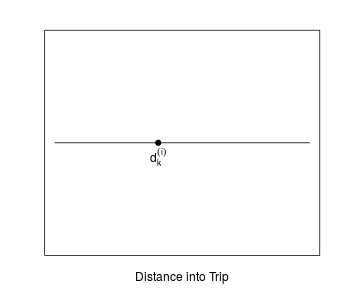
\includegraphics[width=\textwidth]{gps-dist2.png}
    %\caption{}
    \label{fig:gpsdist-1}
  \end{subfigure}
  ~
  \begin{subfigure}{0.4\textwidth}
    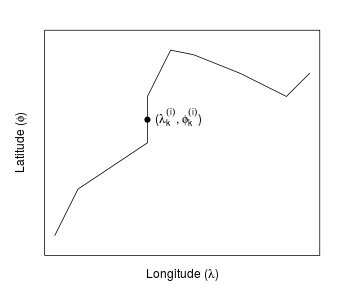
\includegraphics[width=\textwidth]{gps-dist1.png}
    %\caption{}
    \label{fig:gpsdist-2}
  \end{subfigure}
  \caption{%
  Each particle has a value for $d_k^{(i)}$ (left) which can be easily transformed
  to a geographic coordinate (right) using the shape information associated with
  the given route.}
  \label{fig:gpsdist}
\end{figure}

Being able to avoid any unnecessary assumptions or estimations makes the
\pf{} a very attractive candidate for modeling real-time \gls{gps}-based data.
\cite{chen-rakha:2014} used a \pf{} to model travel time in real-time,
and used historical datasets to propose new trajectories for particles.
\cite{hans-etal:2015} also implemented a \pf{} to help model a transit system
in which they wished to devise strategies to solve a particular problem:
to reduce the bunching behaviour of buses along the same route.
They formulated a model which used \emph{headway}, the time delay between
conseutive buses traveling along the same route,
as well as a model for dwell times and traffic signal behaviour.


To predict arrival time using a \pf{}, we can use a similar approach to the transition
function, but instead apply a \emph{prediction function} to each individual particle.
Perhaps the only downside of the \pf{} is the high computational demand,
since we are applying functions to a sample of particles, rather than to
a single state estimate.


Unfortunately, many of the models formulated in the literature use very specific technologies,
and are typically used to target a specific problem.
Not many of them are based on \gls{gps} data alone, 
and therefore are not applicable in a general setting.



% ====================================================================================================== % INFO

% Background knowledge is crucial, therefore describe it fully here.
% Specify the background to the problems you are trying to solve.
% Define anything technical that most statisticians will not be
% familiar with.

% What previous work has been done in the area?
% Cite references relating to such work, e.g.,
% in the form of \cite{reid:2003} and \cite{efro:tibs:1993}.
% Has anybody described any open problems in the literature?

% Make sure that problems arising from the background knowledge
% are clearly described. There should be a logical flow of thought
% in this section starting from the background and leading to the
% problem on hand.

% Don't put anything new in this section.

% ====================================================================================================== % OLD

% Since as early as the 1960's, public transit agencies have been deploying \gls{avl} systems
% in their fleets \citep{tcrp:1997}.
% The purposes of these systems range from operational, such as planning and maintenance, 
% to \glspl{atis}, most notably \gls{rti} and journey planning \citep{tcrp:2003}.
% Most of the early \gls{avl} implementations used a signpost system,
% in which signposts fitted with transmitters would be positioned along a route
% and communicate with passing buses.
% More recently, the \gls{gps} has become increasingly popular as an \gls{avl} technology,
% and is implemented in the Auckland Transport fleet
% and many other fleets around the world.
% For this reason, our work will focus solely on \gls{gps}-based systems.


% In a \gls{gps}-based \gls{avl} system, vehicles report their position to a central server,
% the frequency of which depends on the particular system.
% Usually there is a fixed interval---for example, 30~seconds---between reports,
% although actual frequency can fluctuate due to communication delays and signal interference,
% which can also affect the accuracy of \gls{gps} measurements \citep{cn}.
% If the agency has made it available, 
% these locations can be accessed through public \glspl{api}
% \citep{tcrp:2003}.
% The particular family of \gls{api} we will be working with is \gls{gtfs}
% (see section~\ref{sec:data}),
% which is a globally standardised format for providing transit data to developers
% \citep{gtfs}.
% Having been fitted with an \gls{avl} system, 
% \gls{atis}---which includes arrival time prediction---can be implemented.


% \cite{dailey:2001} implemented a prediction algorithm in Seattle, Washington,
% in which a \gls{kf} (see \cref{sec:kalman_filter}) was used to estimate the state of a bus, 
% which was then used in conjunction with historical data to predict arrival time,
% using a signpost and odometer \gls{avl} system to record the distance travelled along a route.
% \cite{cathey-dailey:2003} released a general prescription for arrival time prediction using
% a \gls{gps}-based system consisting of three parts:
% the first, the ``tracker'', involved converting GPS location to distance into trip measurements
% based on static schedule and shape information;
% the second involved estimating the \emph{true state} of the vehicle (distance into trip, speed, 
% and acceleration) using a \gls{kf};
% and the third presented some alternative arrival time prediction methods and example implementations
% in Seattle and Portland.


% As most of the \gls{kf} arrival time prediction methods were only accurate for
% a few stops ahead \citep{yu-etal:2006},
% many other prediction algorithms were proposed, compared, and implemented
% to varying degrees over the next decade.
% These included data-driven models such as \gls{knn} regression,
% \gls{ann}, and \gls{svm} 
% \citep{chang-etal:2010,jeong-rilett:2005,yu-etal:2006,yu-etal:2010,yu-etal:2011} [!! add more].
% In these, historical data was collected over a period of time using on-board or at-stop recording,
% and then used in combination with
% real-time \gls{avl} data to generate travel and arrival time predictions.
% These methods, in particular \gls{ann} and \gls{svm},
% were shown to give accurate predictions for many stops ahead \citep{cn}.
% However, these typically require large historical datasets to train the model,
% and don't handle unusual situations well \citep{cn}.


% A more recent approach to modeling the state of transit vehicles is the \gls{pf},
% which has been shown in several transportation studies to outperform the \gls{kf}
% \citep{chen-rakha:2014,cn}.
% \cite{chen-rakha:2014} used a \gls{pf} to predict travel times 
% by proposing new particle trajectories from a historical database,
% while \cite{hans-etal:2015} used a particle filter in an operations research setting,
% in which their goal was to propose control strategies to reduce the ``bunching''
% of consecutive buses along a common route.
% In these models, the \gls{avl} data available included actual arrival times, and in their study,
% \cite{hans-etal:2015} also had \gls{apc} and traffic light information, 
% allowing them to construct complex models.
% There does not appear to have been any large-scale implementations of 
% real-time arrival time predictions using a \gls{pf} based solely on \gls{gtfs} real-time data.




% \subsection{Recursive Bayesian Filters}
% \label{sec:recursive}


% Of the several approaches to modeling real-time bus positions discussed above,
% our work will focus on recursive Bayesian filters, in particular the \gls{pf}.
% Recursive Bayesian filters are a class of model which 
% are specially suited to data that is observed and analysed in real-time,
% such as navigation and tracking applications.
% This makes it a suitable choice for bus tracking models.


% The general framework of recursive Bayesian filters consists of an
% underlying Markov process with true state $\bX_k$, which is unknown and unmeasurable.
% The current state $k$ is dependent only on the previous state, $k-1$:
% \begin{equation}
%   \label{eq:markov_state}
%   p(X_k | X_0, X_1, \ldots, X_{k-1}) = p(X_k | X_{k-1}).
% \end{equation}
% However, there is also a \emph{hidden Markov process}
% with state $\bY_k$ that is dependent on $\bX_k$, 
% for which we can make observations.
% In our case, the \emph{true state} is the distance into trip, $d_k$, 
% and speed, $v_k$, of the bus,
% $\bX_k = [d_k\ v_k]^T$, which we cannot observe.
% Instead, the bus reports its GPS position
% (latitude, $\phi$, and longitude, $\lambda$) at regular intervals,
% so the observation state is $\bY_k = [\phi_k\ \lambda_k]^T$.


% There are many different recursive Bayesian filters,
% but the two we will discuss are the \gls{kf} (\cref{sec:kalman_filter}),
% which has been used in many arrival time prediction applications,
% \citep{wall-dailey:1999,dailey:2001,cathey-dailey:2003},
% and the \gls{pf} (\cref{sec:particle_filter}), 
% which is a generalised form and has recently
% shown up in several transit applications 
% \citep{chen-rakha:2014,hans-etal:2015,cn}.



% \subsubsection{Kalman Filter}
% \label{sec:kalman_filter}

% The \gls{kf} has been predominant in 
% many real-time applications which, apart from its use in transit described here,
% include missile guidance systems and the navigational systems of
% the International Space Station \citep{cn}.
% In many applications, the \gls{kf} model is based on linear physics equations,
% such as Newton's Laws of Motion, to predict future position
% given current position, speed, acceleration, and many other inputs \citep{cn}.


% The \gls{kf} works in two steps.
% First, the new state is \emph{predicted} from the previous one,
% and then the state is \emph{updated} using the observations.
% Each state is specified by a mean vector and covariance matrix,
% which represents process noice and measurement error,
% balanced by the algorithm;
% therefore, the state is assumed to have a multivariate normal distribution.


% The \gls{kf} assumes a linear state transition specified by
% a matrix $\mat{A}$, with Gaussian process noise $\mat{w}_k$.
% That is, 
% \begin{equation}
%   \label{eq:kf_statetransition}
%   \bX_k = \mat{A}\bX_{k-1} + \mat{w}_k.
% \end{equation}
% There can also be a control vector for inputs such as turning or acceleration,
% but these are not applicable in our setting so they are left out.
% The relationship between the unknown state and the observable state is described
% by a measurement matrix $\mat{H}$, along with the measurement error $\mat{v}_k$,
% \begin{equation}
%   \label{eq:kf_measurement}
%   \bY_k = \mat{H}\bX_{k-1} + \mat{v}_k.
% \end{equation}
% The limitation here is that the relationship between $\bX$ and $\bY$ needs to be a linear
% combination of the state parameters that can be expressed in a matrix.
% For example, if the observation is of the distance traveled (such as provided by an odometer), 
% the measurement matrix would simply be $\mat{H} = \left[1\ 0\right]$, 
% which extracts the distance from the state vector.


% In the \gls{kf} implementation mentioned earlier,
% \cite{cathey-dailey:2003} were required to first estimate the 
% distance into the trip in their ``tracker'' step to make intermediate ``observations'',
% denote $\bZ_k$, allowing them to use $\mat{H}$ as defined above.
% These approximate observations were used in the update step of the \gls{kf}.
% Along with the assumption of Gaussian errors,
% this makes the \gls{kf} somewhat restrictive,
% and not ideal for modeling processes which do not obide strictly to linear dynamic equations
% (see \cref{sec:busbehavior}).



% \subsubsection{Particle Filter}
% \label{sec:particle_filter}

% In response to the restrictive nature of the \gls{kf}, there have been many 
% alternatives described, such as the Extended Kalman Filter \citep{cn};
% however, we will focus on the \gls{pf}.
% This generalised filter allows the use of \emph{unrestricted functions} to define
% state transitions and measurements, rather than be limited by matrices,
% and makes no unnecessary assumptions about the distributions involved.


% Instead of modeling the state distribution entirely, 
% the \gls{pf} uses a sample of $M$ independent state estimates called \emph{particles}, 
% which can each be modeled individually, and then resampled (with replacement) 
% using the likelihood of each particle to generate sampling weights.
% In our case, we assume a bus has an unknown state $\bX_k = [d_k\ v_k]^T$,
% so each individual particle is denoted $\bX_k^{(i)} = [d_k^{(i)}\ v_k^{(i)}]^T$,
% $i = 1, \ldots, M$.


% \begin{figure}[b]
%   \centering
%   \includegraphics[width=0.45\textwidth]{gps-dist2.jpg}
%   \includegraphics[width=0.45\textwidth]{gps-dist1.jpg}
%   \caption{Relationship between a particle's distance into trip (right) and associated GPS coordinates
%   (left). The single value of distance can be mapped to a GPS coordinate,
%   which can in turn be compared to the observed position.}
%   \label{fig:gps-dist}
% \end{figure}


% When a new observation is recieved,
% we can model each particle individually and independently using the state transition function, $f$,
% applied to the particle's current state,
% as well as any other information we have available (see \cref{sec:busbehavior}) and process noise,
% \begin{equation}
%   \label{eq:pf_statetransition}
%   \bX_k^{(i)} = f(\bX_{k-1}^{(i)}, \ldots, \mat{w}_k^{(i)}).
% \end{equation}


% Since each particle has its own value of $d_k$, 
% we can use the shape information supplied by \gls{gtfs} to
% find the coordinates of that particle (see \cref{fig:gps-dist}).
% Now, instead of generating pseudo-observations of distance
% as in the \gls{kf} approach, we do the reverse: map the unknown state into 
% a space we can compare directly to the observations (i.e., \gls{gps} coordinates):
% \begin{equation}
%   \label{eq:pf_measurement}
%   \bZ_k^{(i)} = h(\bX_k^{(i)}).
% \end{equation}
% The distance between two GPS coordinates (the Great Circle Distance)
% can then be used to generate weights for each particle.
% The weight of the $i^{\mathrm{th}}$ particle is given by
% \begin{equation}
%   \label{eq:pf_likelihood}
%   w_i = \frac{p(\bZ_k^{(i)} | \bY_k)}{\sum_{j=1}^M p(\bZ_k^{(j)} | \bY_k)}
% \end{equation}
% Note that the likelihood uses the distance between the particle and the 
% reported \gls{gps} location.
% These weights are used to resample with replacement, generating a posterior distribution 
% of particles approximating the new state.


% The main advantage of the \gls{pf} is that we make no unnecessary 
% assumptions about the error distributions, 
% and are no longer restricted to linear transitions between states;
% instead, only by computational complexity.
% One of the unique features of modeling bus movement
% is \emph{dwell times},  discussed in \cref{sec:busbehavior},
% which can introduce transitions between states which are conditional on
% how long a bus spends at each stop (which can be zero).
% Multimodality is also common around bus stops, particularly in the proposal distributions, 
% which can be problematic for a \gls{kf} 
% which assumes unimodal distributions for all parameters.


% Another advantage of the \gls{pf} is that it extends easily to the problem of arrival time prediction.
% At any time $k$, we have a posterior distribution for the current state,
% where each particle has its own value for distance and velocity. 
% These particles can be projected forward using state information and historical data
% to obtain a sample of arrival times
% based on a predictive model applied to each particle,
% rather than a full state distribution.
% The predictive distribution makes no assumptions other than those in the model
% used to obtain it.









% \subsection{Modeling Bus Behavior}
% \label{sec:busbehavior}


% One unique feature of modeling bus behaviour is that 
% they can stop and wait at bus stops along the route
% while passengers get on and off.
% The time spent waiting at a stop is known as \emph{dwell time},
% and has been shown to be necessary in accurately modeling bus behavior \citep{cn}.
% It can be rather complicated to implement dwell times into a \gls{kf} framework,
% so most of them only seem to implement dwell times in the arrival time prediction part.
% The PF, however, has no difficulty in dealing with dwell times,
% and \cite{hans-etal:2015} describe how they applied a such a model
% to the transit system in Portland, Oregon.


% When approaching a bus stop,
% each particle can independently decide whether or not it will stop,
% and depending on the outcome follow the relevant trajectory.
% Those particles that do stop will each be given (independently)
% a dwell time, after which period they continue along the route.
% Inevitably, when passing a stop, the prior distribution of the particles will be multimodal:
% those that stopped, and those that didn't.
% The stopping probabilities can be modeled based on historical data,
% but separately from the main algorithm to reduce computations.

% \begin{figure}[bt]
%   \centering
%   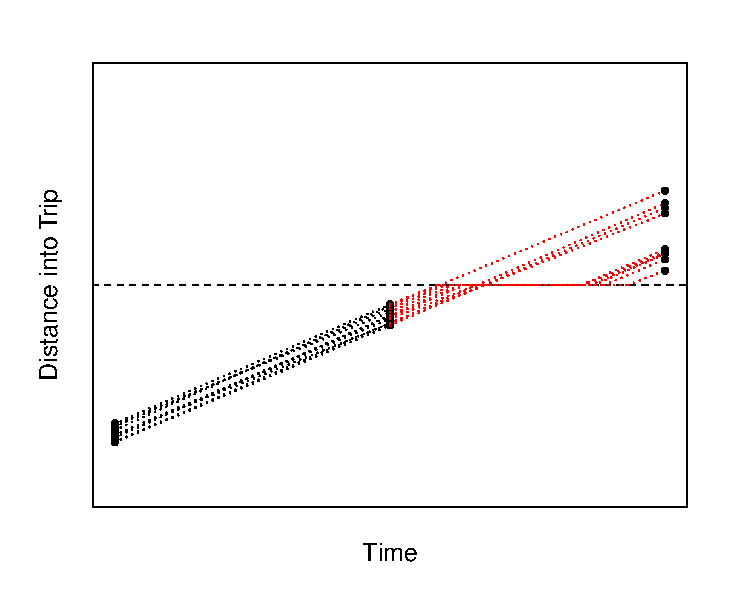
\includegraphics[width=0.6\textwidth]{particle-stop.pdf}
%   \caption{Multimodal proposal distribution of particles when passing a stop.}
%   \label{fig:particle-stop}
% \end{figure}

% Other features somewhat unique to bus tracking, 
% in contrast to traditional tracking algorithms,
% is that they follow known paths, at known times of the day \citep{cathey-dailey:2003}.
% We have departure times, stop locations, 
% and various other details which we can---and should---make use of 
% when formulating our models.
% An example where route information is used is when multiple buses travel the same 
% route at various times of the day (known as trips).
% Several implementations have used this concept in their models.
% \cite{yu-etal:2011} took this idea further but noticing that some routes would 
% travel past the same stops at the beginning or end of the route.
% They proposed a model that used the travel time of between stops based on buses 
% from multiple different routes, and showed that it improved the accuracy of 
% predictions compared to using just a single route.
% However, this was limited to routes along a freeway,
% and only looked at routes using the same stops.
% There are some situations where buses will travel along the same road ways, 
% but not necessarily stop at the same stops.
% These could, however, be useful for predicting arrival times of subsequent buses.



% \subsection{Predicting Arrival Time}
% \label{sec:arrivaltimeprediction}

% So far, we have been focussed on modeling the current state of a vehicle in real-time.
% The next part involves using this estimated state to predict arrival times 
% at future stops along the route.
% Arrival time prediction has been evolving since some of the first \gls{avl}
% systems were installed in bus fleets.
% Prediction methods range from schedule deviation \citep{cn},
% to more complicated prediction functions involving historical data,
% dwell times, and headway on routes with multiple buses 
% \citep{cn}.


% Some of the simpler, early models used either scheduled arrival times, 
% or else data sets collected over a period of time which were then used to 
% compute average speed or travel times between stops.
% This was then used to predict future travel and arrival times;
% however, they were typically only reliable for a few stops ahead \citep{cn}.
% \cite{cathey-dailey:2003} used more complex predictive models, 
% which were capable of incorporating historical travel time
% data---including, for example, weather effects---to predict 
% future travel and arrival times.


% There has also been a significant amount of work on data-intensive models,
% which rely on historical patterns to make travel and arrival time predictions.
% One of these is \gls{knn}, which uses the closest matching historical observations
% to make predictions \citep{cn}.
% Other computer learning models, such as \gls{ann} and \gls{svm}, have also been shown to
% provide accurate predictions that aren't only limited to a few stops ahead
% \citep{cn}.


% Several studies have used the concept of \emph{headway},
% which is the time difference between consecutive buses traveling along the same route.
% In these, travel times of the most recent bus along the same route can be used
% to predict future travel times of the current bus, and therefore arrival times.
% \cite{yu-etal:2011} took this a step further and were able to use travel times
% from multiple \emph{different routes} that all used the same stops in one part of the route.
% They showed that this was more accurate than using just a single route;
% [however, they used \gls{avl} technologies that recorded actual arrival times,
% and therefore actual travel times between stops,
% and it was restricted to routes that used the same sequence of stops 
% (at least for part of a route).]
% \footnote{???}


% More recently, \cite{hans-etal:2015} used a \gls{pf} to predict arrival time, 
% for which headway was one of their predictors.
% They also included models for dwell times and traffic signals.
% A different approach to using historical data was proposed by \cite{chen-rakha:2014}, 
% who used historical trip trajectories to replace low-weighted particles.
% Their results were promising, however only applied to travel times along a freeway,
% and required several months of data.


% [One common thread in the current literature is that most of the models have been applied to a
% specific \gls{avl} system, rather than to a general \gls{gtfs} feed.
% One likely reason for this is that most of the studies have been funded,
% at least partially, by the transit companies, and so they have had access to data
% that is not usually available through public developer \glspl{api},
% or used special \gls{avl} technologies deployed only for the study,
% and are not usually available.]\footnote{???}

% ====================================================================================================== % ENDOLD

% ----------------------------------------------------------------------
\section{So What's New?}
\label{sec:whatsnew}



% ====================================================================================================== % INFO

% List \textit{specific} and \textit{new} results that your thesis
% plans to obtain, especially with regard to new statistical theory
% and methodology.
% It is essential that you have provided comprehensive background
% (in Section~\ref{sec:background})
% so that it is clear what new contributions will be made (here),
% and how they will extend what is currently known.
% Tie these with Appendix~A(i), and a list such as below is a
% good idea.


% For example, all of the points below are new (to my knowledge)
% and have not been done yet.
% \begin{enumerate}

% \item
% Develop a new method for quantile regression based on the
% asymmetric Laplace distribution and the concept of link functions
% and parallelism assumptions (via constraint matrices).


% \item
% Derive the asymptotic properties of the above method,
% both as $n \rightarrow \infty$ and as $p \rightarrow \infty$.




% \item
% Conduct a small simulation to check the mean squared error and
% other properties. To be done in R with some sections written in~C
% calling LINPACK \citep{dong:bunc:mole:stew:1979} for additional speed.



% \item
% Compare my results to those of~\cite{wei:carr:2009}, especially
% relating to boundary effects and small-sample properties.



% \item
% Tackle an important dataset or problem that no one has
% satisfactorily resolved before. It is essential that new
% methodologies are investigated and that novel insights are
% obtained. Note that a conventional analysis, even of a very large
% dataset, is \textit{not} PhD-level research.


% \end{enumerate}

% ====================================================================================================== % OLD

% This work will consist of three main parts:
% real-time bus modeling using a particle filter,
% arrival time prediction using a combination of the particle filter,
% historical data, and ``real-time'' travel time information
% from other buses,
% and finally methods of providing this information to commuters,
% including prediction intervals
% to display uncertainty and journey planning applications.



% \subsection{Particle Filtering}
% \label{sec:new-pf}

% Unlike several other studies, including those by \cite{hans-etal:2015},
% we will be working with only GTFS (realtime) data provided by Auckland Transport.
% One big difference between this data and many others is that we do not have
% actual arrival times available.
% Similar to a standard \gls{mcmc} algorithm, we obtain a posterior sample from the posterior
% distribution, represented by the particles.
% Each particle will have its own values for the parameters,
% which we can expand to include arrival time at the previous stop.
% That is, when a particle passes a stop, it's arrival time is recorded in its state.
% We can then use these arrival times to obtain a posterior distribution of arrival times
% for a bus at a given stop.


% There are several situations we hope the \gls{pf} will be able to improve on.
% The first is dwell times, which was mentioned in \cref{sec:busbehavior}, 
% and was shown in several cases to be necessary in models \citep{cn}, 
% and easily implemented using a \gls{kf} \citep{hans-etal:2015}.
% Another is reliability at loops:
% several routes in the \gls{at} network have \emph{loops},
% in which, given a \gls{gps} coordinate, the bus could either be
% at the beginning (heading into) the loop, or at the end of (heading out of) a loop.
% In a \gls{kf} approach, we would need to make a best guess as to which situation 
% the bus is in; 
% in a \gls{pf}, however, we can just allow some of the particles to be in one state
% and the rest in the other;
% in fact, no extra conditions or logic are required.

% [[ FIGURE of loop? ]]




% \subsection{Prediction}
% \label{sec:new-prediction}


% Improving bus arrival time prediction is the primary goal of this work.
% As we will already have a posterior distribution for the current state of
% each bus, 
% we will be able to use this---along with any other information we
% have available---to predict arrival time.


% We will be comparing various methods of prediction:
% simple state prediction (that is, using only the current state of the 
% bus to predict arrival time),
% which could act as a ``back up'' if all other methods are unavailable,
% historical based prediction,
% real-time traffic conditions obtained from other buses,
% and most likely combinations of these.
% In each of these, we will allow for dwell times at stops along the way.


% In the absense of historical data---for example, in a new system or when
% routes are changed---many models will be unusable until data has been collected.
% In this case, it's good to have a baseline prediction model that can use 
% only the current state, in combination with shedule information,
% to predict arrival times.
% This will be especially useful as the \gls{at} network undergoes
% extensive modifications over the next several years.


% More refined models can be built once data has been obtained, 
% and then used to make predictions based on what happened previously.
% ``Historical'' can refer to previous days or weeks,
% but also to previous \emph{trips} on the same day.
% In many routes around Auckland, there are often multiple trips per day,
% so we can expect the most recent of these to be a good predictor for the current trip.
% Models of this kind exist, however we wish to take it one step further:
% to use travel times from other buses traveling along similar routes
% (i.e., use the same roads) but aren't identical.
% This will be especially useful on routes that run less frequently,
% as we will be able to obtain near-real-time traffic information.


% [[ More ... ? ]]



% \subsection{Commuter Information and Journey Planning}
% \label{sec:commuter-info}


% The end goal of our work will be a free web application available to
% commuters, allowing them to check the status of their bus,
% and get information regarding the estimated time of arrival.
% We will investigate point estimates, as well as interval estimates to do this.


% Additionally, providing ETA to destination will also be useful,
% and this will pave the way for journey planning.
% This is where users can enter a start and end location,
% and be shown various routes they can take,
% with estimates of travel time and arrival time,
% allowing them to make informed decisions based on the requirements of their journey:
% arrive on time or arrive as soon as possible?

% ====================================================================================================== %

% ----------------------------------------------------------------------
\section{Data and Special Needs}
\label{sec:data}



% ====================================================================================================== % INFO

% Almost all Statistics PhD theses should analyse at least one
% data set, even if it is a toy data set.


% State their source fully.
% If new data is important to the thesis describe what's new.
% Why is this data set important?
% What is novel about it?
% Specify any ethics or confidentiality issues.


% A plot of some of the data may be useful;
% see Figure~\ref{fig:myfig}.


% Do you have any special needs such as IT needs?
% These include hardware (supercomputing facilities),
% and expertise/technical knowledge.
% Often extra large data sets have special needs associated
% with its processing.
% How do you invisage those needs to be met?



% Funding: anything to report here?
% If your thesis work involves experiments, travel or special
% resources in order to collect data, or essential collaboration with
% experts in your field, then you should describe these requirements
% here along with how you, or your supervisor, will fund these
% requirements. Departments work on tightly planned budgets and
% generally do not have the facilities to pay for unplanned PhD
% related expenses.



% If ethics approval(s)/permissions is needed then put
% any details here.





% \begin{figure}[tt]
% \begin{center}
% %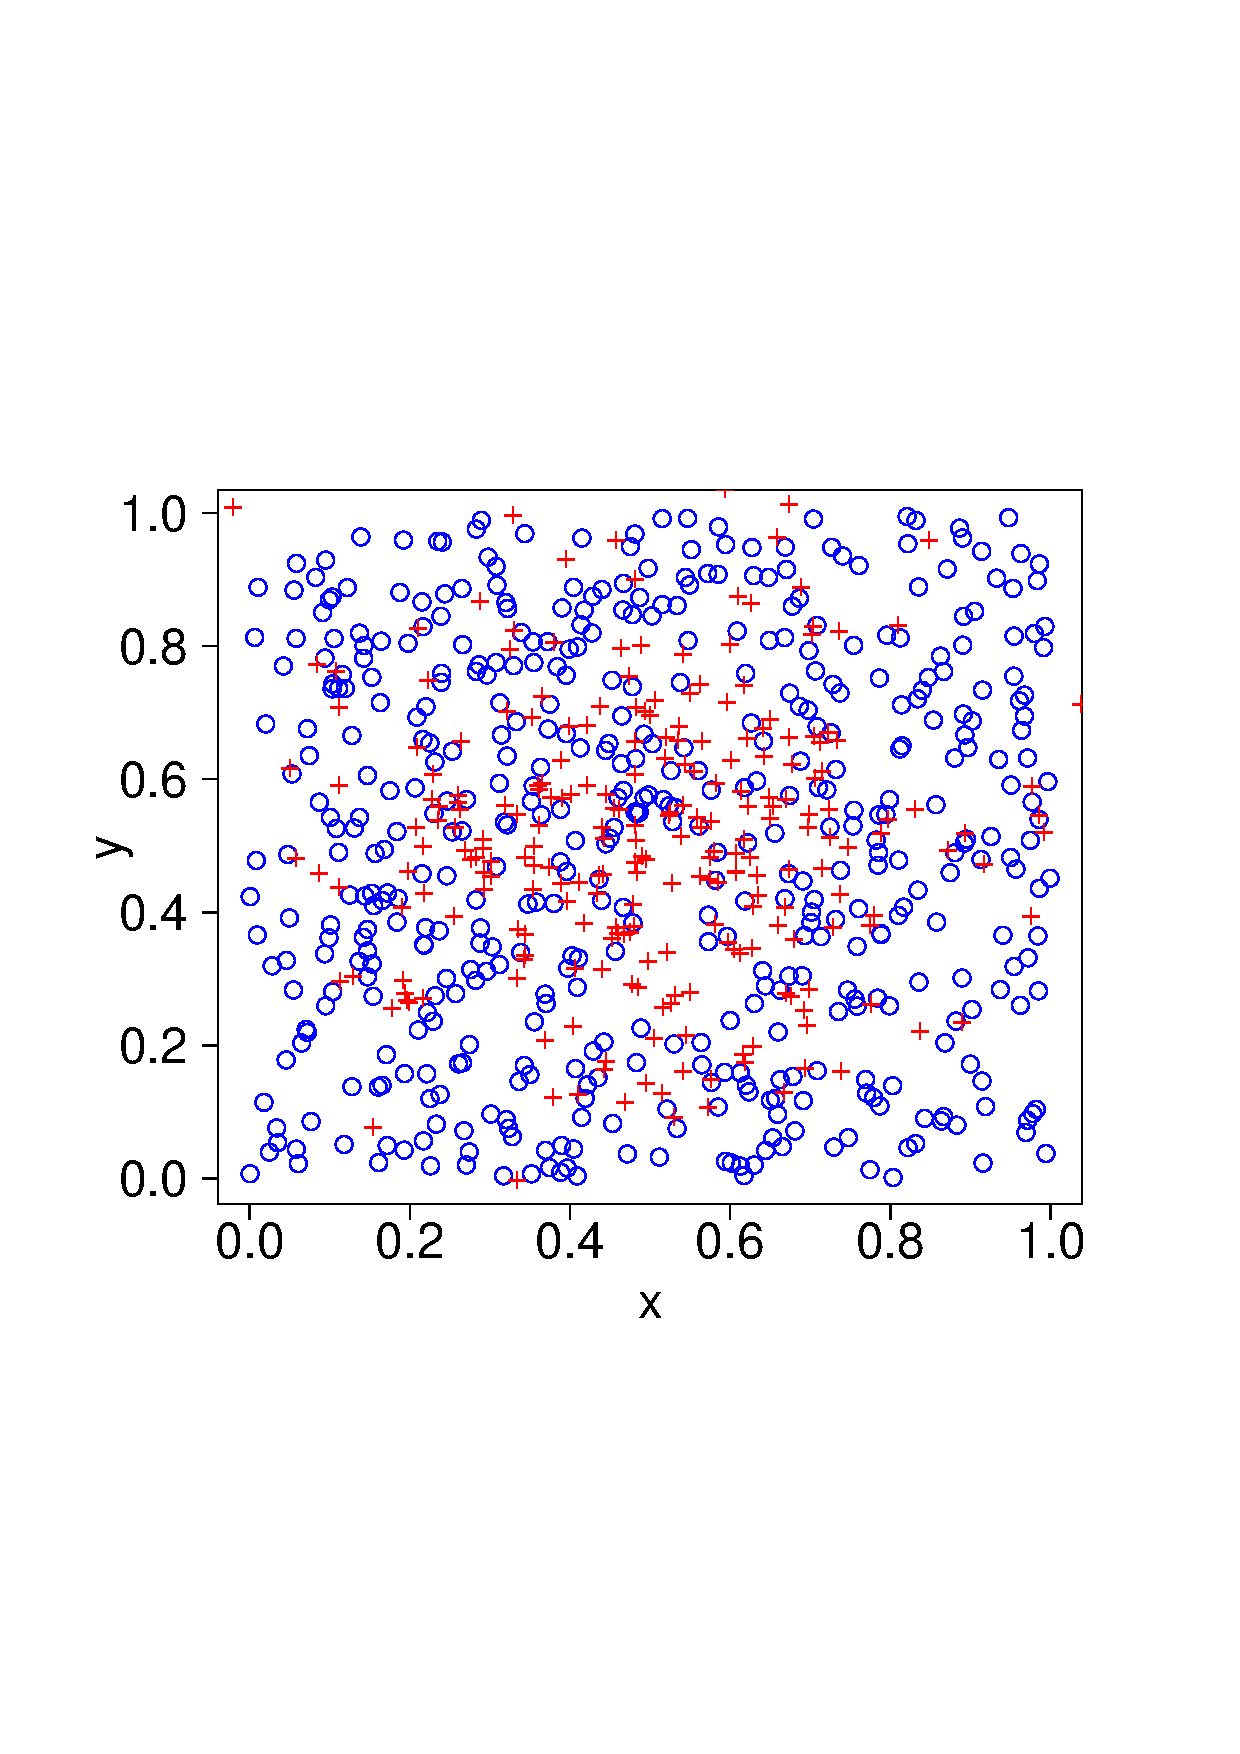
\includegraphics[height=70mm]{./myfig.pdf}
% \caption{
% Data for a two-class classification problem.
% The red ``+'' is for class~1, and $n = 250$.
% The blue ``o'' is for class~2, and $n = 500$.
% }
% \label{fig:myfig}
% \end{center}
% \end{figure}

% ====================================================================================================== % OLD

% Throughout our work, we will be working will publicly available (via API keys) \gls{gtfs}
% (-realtime) data.
% The specification itself is maintained by Google, 
% while the feed we will be using is provided by Auckland Transport.
% This is available at \url{https://dev-portal.at.govt.nz}.
% \gls{gtfs} consists of two parts:
% the static data, which contains information about schedules, trips, stop locations,
% and route shapes, as well as a real-time feed, which gives the most recent locations
% of all buses in the Auckland Transport fleet (over 1000 at peak times).


% Additionally, we will need to store our own historical records of travel times and other
% variables for use in our prediction models. 
% This will likely be in a database, although the exact details of this are yet unknown.


% Due to the computer intensive nature of our work, 
% when we come to deploying a full-scale implementation,
% we will require a dedicated server that can request vehicle positions,
% run the \gls{pf} algorithm,
% and update the predicted arrival times of all buses at future stops.
% We will also require a websever to make these predictiosn available to the public.

% ====================================================================================================== % END OLD


% ----------------------------------------------------------------------
\section{Goals}

% ====================================================================================================== % INFO

% List \textit{specific} goals you wish to achieve in your PhD.


% \begin{enumerate}

% \item
% I wish to derive the first three moments of the Slash distribution.
% This will involve working out the characteristic function first.


% \begin{itemize}

% \item[a.]
% Then work out the observed information matrix
% based on~\cite{bick:etal:2009}.

% \item[b.]
% Then work out the expected information matrix
% \citep{scot:lee:wild:2007}.

% \item[c.]
% Apply the EM algorithm \citep{demp:lair:rubi:1977} to estimate~$\lambda$.

% \item[d.]
% Write a R package to implement my method.
% It will be written in S4 and use object oriented methods
% \citep{cham:1998}.

% \item[e.]
% Apply the method to the radiation data set
% \citep{MR2526777}.

% \item[f.]
% Extend biplots \citep{gowe:1966} for my data.

% \item[g.]
% Release the package on CRAN
% (cf.~\cite{murr:ihak:2000}).

% \item[h.]
% Publish my results in at least two papers,
% earmarked for JASA and JRSS-B.
% Also an applications paper in Biometrics.
% See Section~\ref{sec:timeline}.

% \end{itemize}



% \item
% Solve the Fisher-Behrens problem
% \citep{efro:2009,MR2415600,MR2508377}.


% \end{enumerate}

% ====================================================================================================== %

\begin{enumerate}
\item 
  Implement a Particle Filter on a data set and make predictions that are on par with those currently available.

\item 
  Investigate ways of using other live and historical data to improve the accuracy of estimates.

\item 
  Look at different summary statistics for better point-estimates, and look into providing useful prediction intervals.

\item 
  Implement a large-scale version of the model for a (subset of) the AT PTS, and see how well it runs.

\item 
  Create a web/phone app to access the predictions.

\item
  Package the system so that it is distributable to other feeds to remove its dependency on us.
\end{enumerate}






% ----------------------------------------------------------------------
\section{Timeline and Activities}
\label{sec:timeline}

% ====================================================================================================== % INFO

% \begin{table}[hh]
% \caption{
% Timeline of my privisional year.
% }
% \centering
% \ ~~~~ \\
% \label{tab:timeline}
% \begin{tabular}{|c|l|}
% \hline
% Date & Activity \\
% \hline
% 2010-04-01 & Provisional PhD registration (PhD in Statistics). \\
% 2010-05-01 & Updated my personal webpage at
%              \textsf{www.stat.auckland.ac.nz/$\sim$myStudentName}. \\
% 2010-05-20 & Attended one of the
%              Doctoral Skills Programme's Induction Days. \\
% 2010-09-01 & Gave my first talk at NZSA conference. Won first prize. \\
% 2010-11-01 & Gave a talk to PhD Talks Day. \\
% 2011-01-15 & Submit my first paper to \textit{Annals of Statistics}
%              (co-authored with supervisor). \\
% 2011-05-01 & Presented my research progress to a departmental seminar. \\
% 2012-01-20 & Achieve Goal~1. \\
% 2012-08-20 & Achieve Goal~2. \\
% 2012-10-23 & Submit my second paper to \textit{Annals of Applied Statistics}
%              (co-authored with supervisor). \\
% 2013-01-15 & Submit my third paper to \textit{Biometrics}
%              (sole authorship). \\
% 2013-02-01 & Submit my PhD thesis. \\
% \hline
% \end{tabular}
% \end{table}

% ====================================================================================================== %

I have fulfulled all my first year requirements.
These are:
\begin{enumerate}

\item
All EoI provisional goals:
\begin{enumerate}

\item
\textit{Approval of the full thesis proposal by the appropriate departmental/faculty postgraduate
committee}:
Here it is!

\item
\textit{A substantial piece of written work, such as a literature review, completed to the
satisfaction of the main supervisor}: Here?


\item
\textit{Presentation of the proposal and/or work in progress to an appropriate forum e.g.\ seminar,
research group, conference, to the satisfaction of the supervisors}:
YYYY-MM-DD.

\item
\textit{Attendance at one of the Doctoral Skills Programme
Induction Days}:
2015-11-04

\item
\textit{Successful completion of the Academic Integrity Module}:
dd/mm/2014

\item
\textit{Undertake Diagnostic English Language Needs Assessment (DELNA) online screening}:
25/02/2010

\item
\textit{Complete STATS 710 and STATS 769 at B+ or higher grade within the first 
12~months\footnote{STATS 769 taught second semester, unable to complete within 12~months}
of registration}

\item
\textit{Attendance of at least 10~Statistics departmental research seminars per annum, 
with forms fully filled in and handed in}:
see Table~\ref{tab:seminars}

\item
\textit{Maintenance of a personal departmental webpage providing information on scholarly
activities and objectives to the satisfication of the supervisor and Department of Statistics
PhD Officer}:
\url{https://www.stat.auckland.ac.nz/people/tell029}

\item
\textit{Satisfactory participation in the Department of Statistics PhD Talks Day and/or give
a departmental seminar within the first 12~months of registration}:
(c)


\end{enumerate}





% \item
% I have updated my webpage
% (\textsf{www.stat.auckland.ac.nz/$\sim$myStudentName})
% giving details of my thesis, links to other research resources
% in my topic, and some personal stuff to make it interesting.


% \item
% I have diligently attend as many Statistics Department seminars
% as I could. They are given in Table~\ref{tab:seminars}.
% This is much more than the minimum quota set by the department.
% Consequently there should be no problem due to this when getting
% my annual report signed off\footnote{If insufficient seminars have
% been attended then sign off will occur \textit{after} the minimum number
% is reached.}.
% The 2010-04-08 seminar was particularly useful because it gave
% me an idea on how to solve one of my problems.


% \item
% I did STATS~730 in Semester~1 of 2010 and obtained an A+.


% \item
% I did STATS~782 in Semester~2 of 2010 and obtained an A.



\end{enumerate}











\begin{table}[hh]
\caption{
Departmental seminars I have attended.% (top part of the table).
%Talks from another UoA departments are in the middle tier.
%Conferences and workshops are in the bottom tier.
}
\centering
\ ~~~~ \\
\label{tab:seminars}
\begin{tabular}{cll}
\toprule
Date & Speaker & Title \\
\midrule
2015-09-02 & Moshe Haviv &
Queues \& cooperative games \\
%
2015-11-18 & Hadley Wickham &
Pure, predictable, pipeable: creating fluid interfaces with R \\
%
2016-01-16 & Xudong Huang &
Composite likelihood estimators, mixed models \& complex \\
&&sampling \\
%
2016-01-27 & Kevin Knuth &
Modern probability theory \\
%
2016-01-28 & Maartje an de Vrugt &
Online appointment scheduling: a taxonomy and review \\
%
2016-02-24 & Arndl von Haeseler &
Terraces, partial terraces, and phylogenetic inference \\
%
2016-03-31 & Shengwei Hu &
Classification on high-dimensional data using\\&&nonparametric mixtures \\
%
2016-04-14 & June Lau &
Optimizing the cardiac patient's journey: using mathematical \\
&&modelling to guide patient flow, staffing, scheduling and \\
&&resource allocation through the cardiac unit \\
%
2016-06-01 & Arman Bilge &
Hamiltonian Monte Carlo on the space of phylogenies \\
%
2016-07-13 & Nikki Sonenberg &
Matrix analytic methods for analysing stochastic fluid models \\
%
% \midrule
% 2010-06-16 & James B.~Conant &
% ``Geography is not a university subject'' (geo Department) \\
% %
% yyyy-mm-dd & Speaker Name &
% Title of Talk \\
% \midrule
% 2010-05-29 & David Siegmund &
% Workshop on `Genetic Mapping' at UoA. \\
%
\bottomrule
\end{tabular}
\end{table}




% ----------------------------------------------------------------------
\section{Summary}



% Give a few sentence summary of your thesis, especially
% what's new.



We're gunna make people happy.











% ----------------------------------------------------------------------
\section*{Appendix~A}

% Delete or replace the contents of this section with any
% appendices you may have.

% \bigskip

% \bigskip

% The \textit{University of Auckland Statute and Guidelines for the
% Degree of Doctor of Philosophy (PhD)} (2008)
% reads\footnote{Clause~1, Preamble, item~(d).}:

% \bigskip


% \noindent
% ``The PhD degree is awarded for a formal and systematic
% exposition of a coherent programme of advanced research
% work carried out over the period of registration for the
% degree which in the opinion of the examiners and the Board
% of Graduate Studies satisfies all of the following criteria:

% \begin{itemize}

% \item[(i)] to be an original contribution to knowledge or
% understanding in its field, and

% \item[(ii)] to meet internationally recognised standards
% for such work, and

% \item[(iii)] to demonstrate a knowledge of the literature
% relevant to the subject and the field or fields to which
% the subject belongs, and the ability to exercise critical
% and analytical judgement of it, and

% \item[(iv)] to be satisfactory in its methodology, in the
% quality and coherence of its written expression, and in
% its scholarly presentation and format.''

% \end{itemize}





\addcontentsline{toc}{section}{References}
\bibliographystyle{./elsart-harv} % elsart-harv,plain,unsrt,alpha
\bibliography{./myrefs}


\end{document}


